%
\chapter{Commutation de paquets}
%
    \section{Un commutateur de paquets}
%
        \subsection{Énoncé}
%
            \paragraph{}
Nous cherchons à simuler un lien de sortie d'un commutateur de paquets.
%
            \begin{figure}[h]
                \centering
                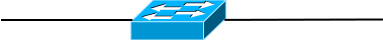
\includegraphics[scale=0.7]{RSC/2-0.png}
                \caption{ Schéma du système à commutateur de paquets étudié }
                \label{ Schema du systeme a commutateur de paquets }
            \end{figure}
%
            \paragraph{}
L'arrivée des paquets est supposée suivre une loi exponentielle de paramètre $\lambda$.
Nous positionnons une file en sortie du commutateur pour stocker les différents paquets.
Les paquets ont une longueur exponentiellement distribuée de paramètre $\frac{1}{\nu} = 10 \ \text{Kb}$.
Le lien de sortie a un débit de $10 \ \text{Mb}.\text{s}^{-1}$.
%
%
        \subsection{Calcul analytique du temps moyen de service $\frac{1}{\mu}$}
%
                \paragraph{}
On obtient le même temps moyen de service suivant :
%
            \[  \text{Temps moyen de service} = \frac{1}{\mu} \]
            \[ \iff \frac{1}{\nu} * \frac{1}{D} = 10 * 10^{3} * \frac{1}{10^{7}} \]
            \[ \iff 10^{4} * 10^{-7} = 10^{-3} \ \text{seconde} \]
%
%
        \subsection{Déterminer le nombre moyen de paquets dans la file et le temps moyen de réponse en fonction du taux d'arrivée pour différentes durées de simulation}
%
            \begin{figure}[h]
                \centering
                
\includegraphics[scale=0.7]{RSC/2-1.png}
                \caption{ Schéma de fonctionnement d'un commutateur de paquets }
                \label{ Schema de fonctionnement d'un commutateur de paquets }
            \end{figure}
%
            \[  \lambda = \rho * \mu \]
            \[  \text{Charge de trafic} \ \rho = \frac{\lambda}{\mu} \]
            \[  \text{Nombre moyen de client(s) en file d'attente} \ \bar{N} = \frac{\rho}{(1 - \rho)} \]
            \[  \text{Temps moyen de réponse} \ \bar{W} = \frac{1}{(\mu - \lambda)} \]
            \[  \bar{N} = \lambda \bar{W} \]
%
            \begin{center}
                \begin{tabular}{ | c | c| c | c | }
                    \hline
                        $\rho$                                          & 0.1       & 0.5           & 0.9           \\
                    \hline
                        $\lambda$                                       & $10^{2}$  & $5 * 10^{2}$  & $9 * 10^{2}$  \\
                    \hline
                        Nombre moyen de client(s) en file d'attente     & 0.11111   & 1             & 9             \\
                    \hline
                        Temps moyen de réponse [s]                      & 0.00111   & 0.002         & 0.01          \\
                    \hline
                \end{tabular}
            \end{center}
%
%
\clearpage
%
%
        \subsection{Comparaison du résultat de la simulation avec la théorie}
%
            \paragraph{}
Blablabla 1
%
            \begin{figure}[h]
                \centering
                \begin{gnuplot}[terminal=epslatex, terminaloptions=color dashed]
                set xlabel 'Charge (\%)'
                set ylabel 'Taux de rejet / Temps de traitement'
                plot "qnap/partie2/p2.q3.data"  u 1:2 t         "min du temps traitement",\
                    "qnap/partie2/p2.q3.data"   u 1:3 t         "max du temps traitement",\
                    "qnap/partie2/p2.q3.data"   u 1:4 w l t     "moyenne du temps traitement",\
                    "qnap/partie2/p2.q3.data"   u 1:5 t         "min nombre de paquets en attente" axes x1y2,\
                    "qnap/partie2/p2.q3.data"   u 1:6 t         "max nombre de paquets en attente" axes x1y2,\
                    "qnap/partie2/p2.q3.data"   u 1:7 w l t     "moyenne nombre de paquets en attente" axes x1y2
                \end{gnuplot}
                \caption{Résultats de la simulation.}
                \label{pic:p2q3}
            \end{figure}
%
%
\clearpage
%
%
        \subsection{Cas où les paquets ont une taille fixe de $10 \ \text{Kb}$}
%
            \subsubsection{Calculer analytiquement le temps moyen de service $\frac{1}{\mu}$}
%
                \paragraph{}
On obtient le même temps moyen de service que précédemment :
%
                \[  \text{Temps moyen de service} = \frac{1}{\mu} \]
                \[ \iff \frac{1}{\nu} * \frac{1}{D} = 10 * 10^{3} * \frac{1}{10^{7}} \]
                \[ \iff 10^{4} * 10^{-7} = 10^{-3} \ \text{seconde} \]
%
%
            \subsubsection{Résultats en fonction du taux d'arrivée pour différentes durées de simulation}
%
% voir pour trouver des formules, la progression doit être linéaire en fonction de $\rho$.
                \paragraph{}
Blablabla 2
Temps moyen de réponse et nombre moyen de paquets dans la file d'attente :
%
            \[  \lambda = \rho * \mu \]
            \[  \text{Charge de trafic} \ \rho = \frac{\lambda}{\mu} \]
            \[  \text{Nombre moyen de client} \ \bar{N} = \frac{\rho}{2 * (1 - \rho)} \]
            \[  \text{Temps moyen de reponse} \ \bar{W} = \frac{1}{2 * (\mu - \lambda)} \]
            \[  \bar{N} = \lambda \bar{W} \]
%
            %~ \begin{center}
                %~ \begin{tabular}{ | c | c| c | c | }
                    %~ \hline
                        %~ $\rho$ & 0.1 & 0.5 & 0.9 \\
                    %~ \hline
                        %~ $\lambda$ & $10^{2}$ & $5 * 10^{2}$ & $9 * 10^{2}$ \\
                    %~ \hline
                        %~ Nombre moyen de client & 0.11111 & 1 & 9 \\
                    %~ \hline
                        %~ Temps moyen de réponse [s] & 0.00111 & 0.002 & 0.01 \\
                    %~ \hline
                %~ \end{tabular}
            %~ \end{center}
%
%
            \subsubsection{Analyse et comparaison des résultats}
%
                \paragraph{}
Blablabla 3
% TODO >>> SIMULATION ici graphique
                \begin{figure}[h]
                    \centering
                    \begin{gnuplot}[terminal=epslatex, terminaloptions=color dashed]
                    set xlabel 'Charge (\%)'
                    set ylabel 'Taux de rejet'
                    plot "qnap/partie2/p2.cst.data" u 1:2 t "minT",\
                        "qnap/partie2/p2.cst.data" u 1:3 t "maxT",\
                        "qnap/partie2/p2.cst.data" u 1:4 w l t "moyenne temps traitement",\
                        "qnap/partie2/p2.cst.data" u 1:5 t "minA" axes x1y2,\
                        "qnap/partie2/p2.cst.data" u 1:6 t "maxA" axes x1y2,\
                        "qnap/partie2/p2.cst.data" u 1:7 w l t "moyenne nb paquets en attente" axes x1y2
                    \end{gnuplot}
                    \caption{Résultats de la simulation pour des paquets à la taille fixe de $10 \ \text{Kb}$.}
                    \label{pic:p2cst}
                \end{figure}
%
%
    \clearpage
%
